% Этот шаблон документа разработан в 2014 году
% Данилом Фёдоровых (danil@fedorovykh.ru) 
% для использования в курсе 
% <<Документы и презентации в \LaTeX>>, записанном НИУ ВШЭ
% для Coursera.org: http://coursera.org/course/latex .
% Исходная версия шаблона --- 
% https://www.writelatex.com/coursera/latex/5.1

\documentclass[t]{beamer}  % [t], [c], или [b] --- вертикальное выравнивание на слайдах (верх, центр, низ)
%\documentclass[handout]{beamer} % Раздаточный материал (на слайдах всё сразу)
%\documentclass[aspectratio=169]{beamer} % Соотношение сторон

%\usetheme{Berkeley} % Тема оформления
%\usetheme{Bergen}
%\usetheme{Szeged}

%\usecolortheme{beaver} % Цветовая схема
%\useinnertheme{circles}
%\useinnertheme{rectangles}
\geometry{paperwidth=140mm,paperheight=105mm}

\usepackage[absolute,overlay]{textpos}

\setbeamercolor{framesource}{fg=gray}
\setbeamerfont{framesource}{size=\tiny}

\newcommand{\source}[1]{\begin{textblock*}{4.2cm}(8.5cm,8.6cm)
    \begin{beamercolorbox}[ht=0.5cm,right]{framesource}
        \usebeamerfont{framesource}\usebeamercolor[fg]{framesource} Source: {#1}
    \end{beamercolorbox}
\end{textblock*}}
\usepackage[absolute,overlay]{textpos}

\usetheme[compress]{Berlin}
\defbeamertemplate*{headline}{miniframes theme no subsection}
{%
  \begin{beamercolorbox}[colsep=1.5pt]{upper separation line head}
  \end{beamercolorbox}
  \begin{beamercolorbox}{section in head/foot}
    \vskip2pt\insertnavigation{\paperwidth}\vskip2pt
  \end{beamercolorbox}%
  \begin{beamercolorbox}[colsep=1.5pt]{lower separation line head}
  \end{beamercolorbox}
}

\setbeamertemplate{footline}[miniframes theme no subsection]
\setbeamertemplate{footline}
{%
  \leavevmode%
  \hbox{\begin{beamercolorbox}[wd=.5\paperwidth,ht=2.5ex,dp=1.125ex,leftskip=.3cm plus1fill,rightskip=.3cm]{author in head/foot}%
     \usebeamerfont{author in head/foot}\insertshortauthor
  \end{beamercolorbox}%
  \begin{beamercolorbox}[wd=.5\paperwidth,ht=2.5ex,dp=1.125ex,leftskip=.3cm,rightskip=.3cm plus1fil]{title in head/foot}%
     \usebeamerfont{title in head/foot}\insertshortinstitute
  \end{beamercolorbox}}%
  \vskip0pt%
}


%%% Работа с русским языком
\usepackage{cmap}					% поиск в PDF
\usepackage{mathtext} 				% русские буквы в формулах
\usepackage[T2A]{fontenc}			% кодировка
\usepackage[utf8]{inputenc}			% кодировка исходного текста
% % \usepackage[english,russian]{babel}	% локализация и переносы
\usepackage[english]{babel}	% локализация и переносы
\usepackage[nottoc]{tocbibind}
\usepackage{url}
\usepackage{hyperref}

%% Beamer по-русски
\newtheorem{rtheorem}{Theorem}
\newtheorem{rproof}{Proof}
\newtheorem{rexample}{Example}

% %%% Дополнительная работа с математикой
\usepackage{amsmath,amsfonts,amssymb,amsthm,mathtools} % AMS
\usepackage{icomma} % "Умная" запятая: $0,2$ --- число, $0, 2$ --- перечисление
\usepackage{svg}
\usepackage{marvosym} % \MVRIGHTarrow
\usepackage{stmaryrd} % \shortrightarrow
\usepackage{textcomp}

%% Номера формул
%\mathtoolsset{showonlyrefs=true} % Показывать номера только у тех формул, на которые есть \eqref{} в тексте.
%\usepackage{leqno} % Нумерация формул слева

%% Свои команды
\DeclareMathOperator{\sgn}{\mathop{sgn}}

%% Перенос знаков в формулах (по Львовскому)
\newcommand*{\hm}[1]{#1\nobreak\discretionary{}
{\hbox{$\mathsurround=0pt #1$}}{}}
\setbeamertemplate{navigation symbols}{}

%%% Работа с картинками
\usepackage{graphicx}  % Для вставки рисунков
\graphicspath{{images/}{images2/}}  % папки с картинками
\setlength\fboxsep{3pt} % Отступ рамки \fbox{} от рисунка
\setlength\fboxrule{1pt} % Толщина линий рамки \fbox{}
\usepackage{wrapfig} % Обтекание рисунков текстом

%%% Работа с таблицами
\usepackage{array,tabularx,tabulary,booktabs} % Дополнительная работа с таблицами
\usepackage{longtable}  % Длинные таблицы
\usepackage{multirow} % Слияние строк в таблице

%%% Программирование
\usepackage{etoolbox} % логические операторы

%%% Другие пакеты
\usepackage{lastpage} % Узнать, сколько всего страниц в документе.
\usepackage{soul} % Модификаторы начертания
\usepackage{csquotes} % Еще инструменты для ссылок
%\usepackage[style=authoryear,maxcitenames=2,backend=biber,sorting=nty]{biblatex}

\usepackage{multicol} % Несколько колонок

%%% Картинки
\usepackage{tikz} % Работа с графикой
\usepackage{pgfplots}
\usepackage{pgfplotstable}
% \usepackage[superscript]{cite}
\usepackage{caption}
\captionsetup[table]{labelformat=empty, font=small,skip=1pt, justification=centering} 
\captionsetup[figure]{labelformat=empty, justification=centering}
\usepackage[font=footnotesize,skip=2pt]{caption}
\usepackage{bm}
\usepackage{xcolor}
\usepackage{lipsum}

\setbeamertemplate{footline}{}

\setbeamertemplate{frametitle}
{
    \nointerlineskip
    \begin{beamercolorbox}[sep=0.3cm,ht=1.8em,wd=\paperwidth]{frametitle}
        \vbox{}\vskip-2ex%
        \strut\insertframetitle\strut
        \vskip-0.8ex%
    \end{beamercolorbox}
}

\newcommand\blfootnote[1]{%
  \begingroup
  \renewcommand\thefootnote{}\footnote{#1}%
  \addtocounter{footnote}{-1}%
  \endgroup
}

\renewcommand{\footnoterule}{%
  \kern -1.6pt
  \hrule width 2.2in height 0.5pt
  \kern 0.1pt
}

\setbeamersize{text margin left=3.5mm,text margin right=3.5mm} 

\title{Improved Autoregressive Modeling with Distribution Smoothing}
\author[Махин Артем \\ Кузнецов Михаил]{Mikhail Kuznetsov}
\date{\today}
\institute[МГУ]{CMC MSU}

\begin{document}

\frame[plain]{\titlepage}	% Титульный слайд
\addtobeamertemplate{navigation symbols}{}{%
    \hspace{1em}%
    \
    \scriptsize\tiny\insertframenumber/\inserttotalframenumber
}
\setbeamertemplate{itemize items}[ball]


\section{Recap}
\begin{frame}

Let $\left\{\bm{x}_{1}, \bm{x}_{2}, \ldots, \bm{x}_{N}\right\}$ --- $D$-dimensional i.i.d samples from a continuous data distribution $p_{\text {data }}(\bm{x})$

\begin{exampleblock}{Property}
An autoregressive model decomposes a joint distribution into univariate conditionals \cite{autoreg}:
$$
p(\bm{x})=\prod_{i=1}^{D} p\left(x_{i} \mid \bm{x}_{<i}\right)
$$
\end{exampleblock}

\begin{block}{Goal}
Find $\theta$ --- parameters of the model such that $p_{\theta}(\bm{x}) \approx p_{\text {data }}(\bm{x})$ 
\end{block}

A commonly used approach for density estimation is maximum likelihood estimation (MLE), i.e., by maximizing 
$$
L(\theta) \triangleq \frac{1}{N} \sum_{i=1}^{N} \log p_{\theta}\left(\bm{x}_{i}\right)
$$
\end{frame}

\section{Models}
\begin{frame}[t]{PixelCNN \cite{pixel}}
\vspace{-8ex}
\begin{columns}[t]
\onslide<2->
\begin{column}{.6\textwidth}
\begin{figure}[h]
            \centering
            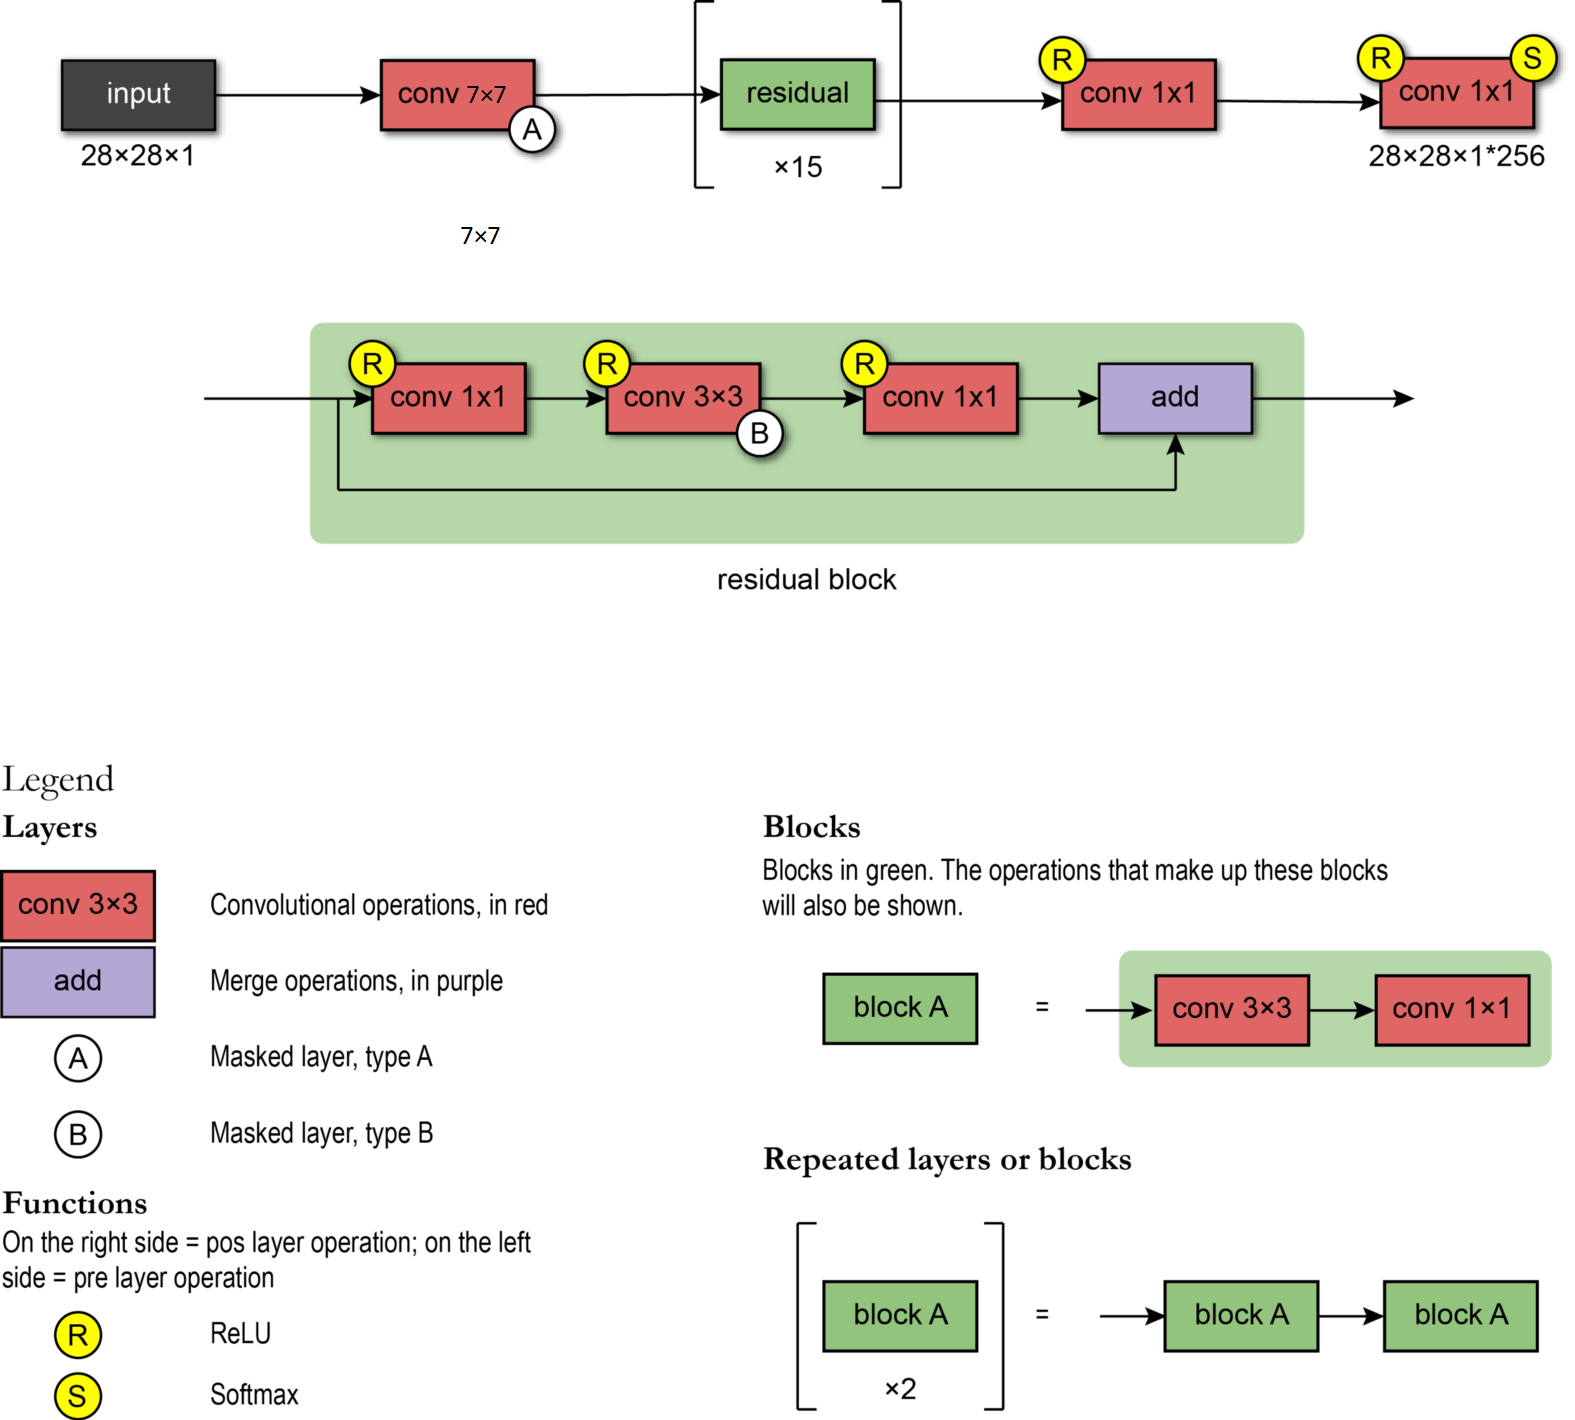
\includegraphics[scale=0.52]{pixelcnn.png}
            \\ \scriptsize Architecture of the PixelCNN
        \end{figure}
\end{column}
\hspace{1mm}
\onslide<1->
\begin{column}{.35\textwidth}
\vspace{5ex}
\begin{figure}[c]
            \centering
            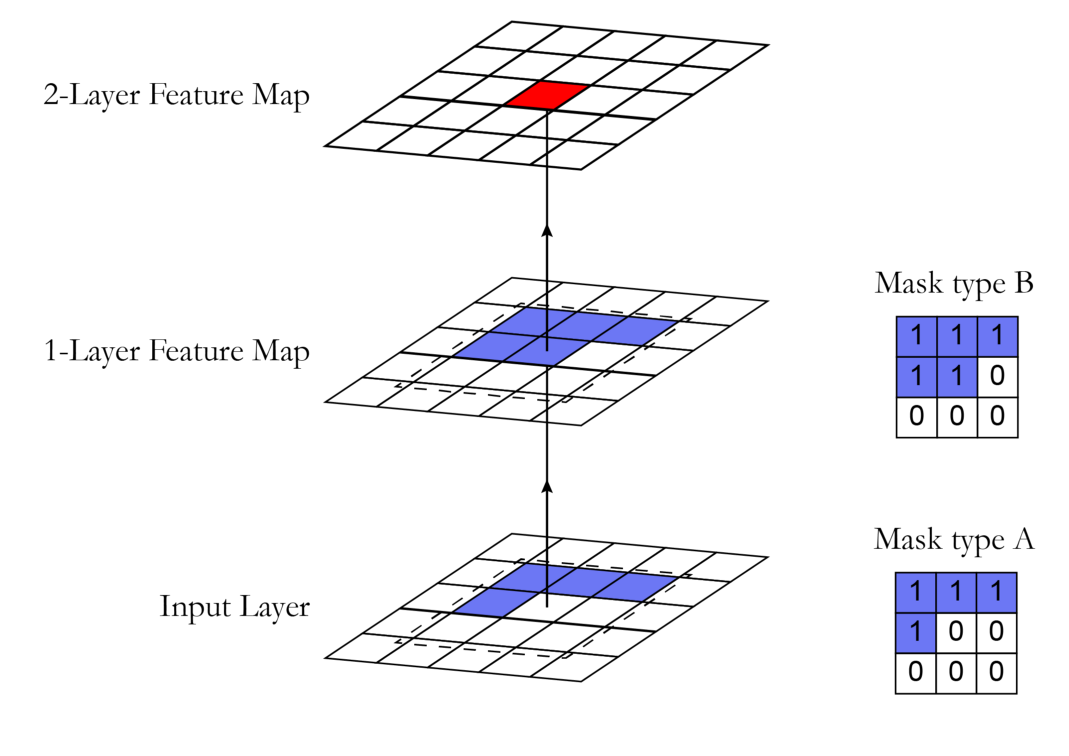
\includegraphics[scale=0.15]{mask1.png}
            \\ \scriptsize Masking 1
        \end{figure}
        \begin{figure}[hp]
            \centering
            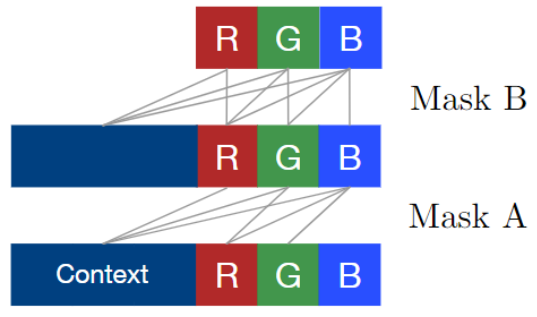
\includegraphics[scale=0.44]{mask2_22.png}
            \\ \scriptsize Masking 2
        \end{figure}
\end{column}
\end{columns}
% \vspace{-10ex}
\scriptsize\blfootnote{\href{https://towardsdatascience.com/autoregressive-models-pixelcnn-e30734ede0c1}{\scriptsize{\textcolor{blue}{Image source}}}}
\end{frame}

\begin{frame}{Gated PixelCNN \cite{conpixel}}
\begin{figure}[hp]
    \centering
    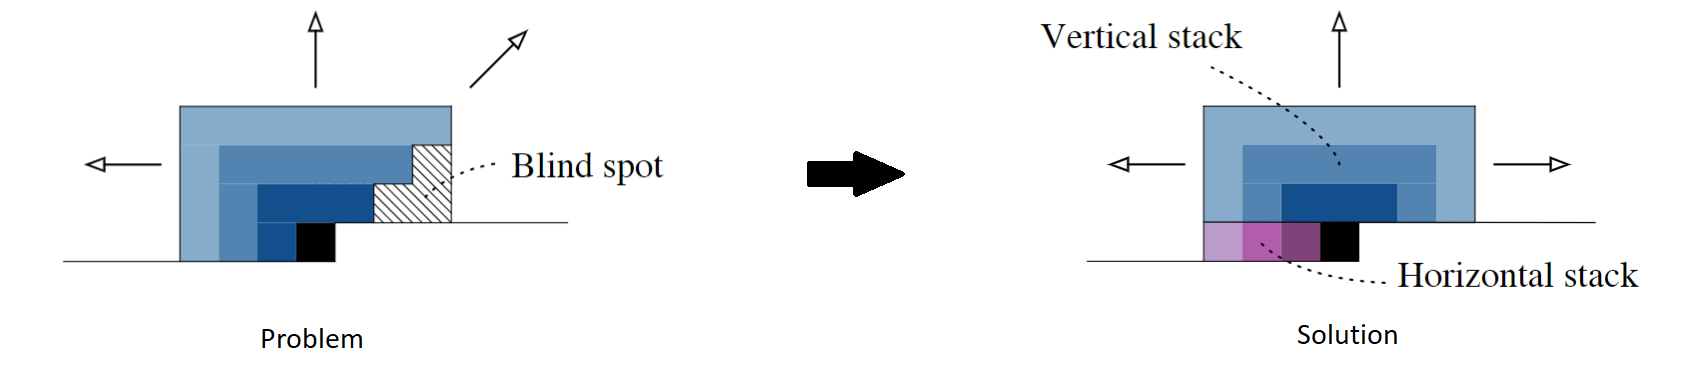
\includegraphics[width=\textwidth]{images/blind.png}
\end{figure}
\pause
\centering
\begin{figure}[hp]
    \centering
    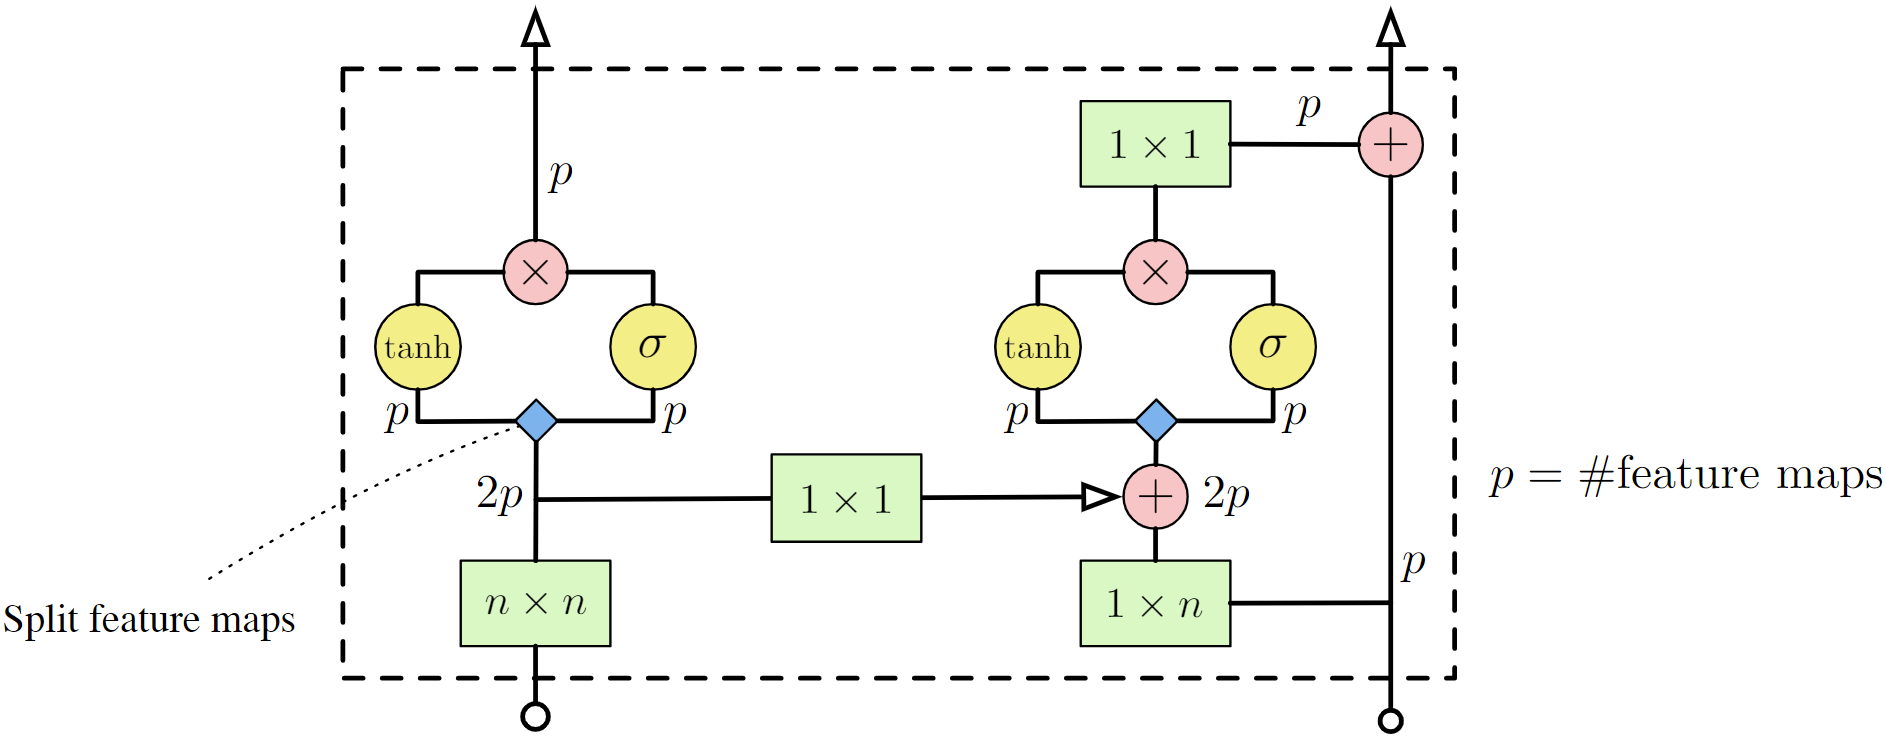
\includegraphics[scale=0.5]{images/gated.png}
    \\ \footnotesize A single layer in the Gated PixelCNN architecture
\end{figure}
\end{frame}

\begin{frame}{PixelCNN++ \cite{pixelplus}}
The most important modifications:
\begin{itemize}
  \pause
  \item  discretized logistic mixture likelihood
  \pause
  \item  conditioning on whole pixels
  \pause
  \item  dilated convolution $\shortrightarrow$ convolution with stride
  \begin{figure}[hp]
    \centering
    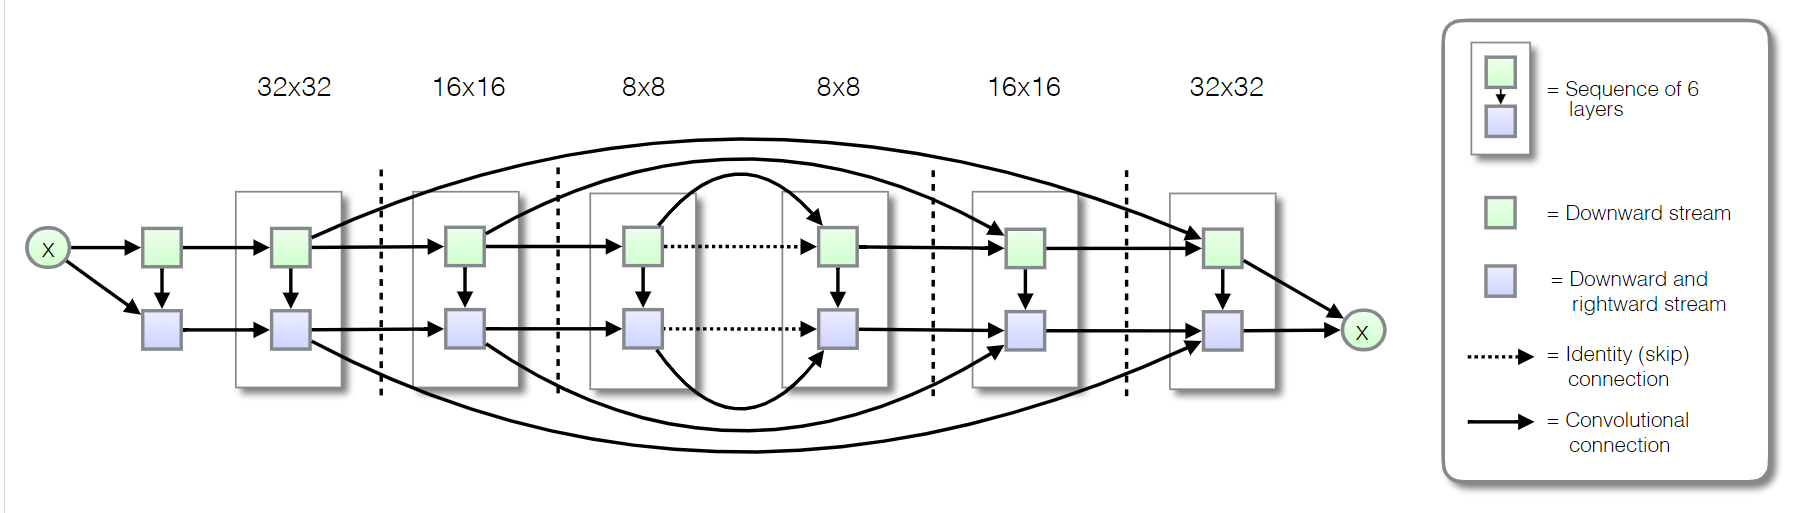
\includegraphics[scale=0.6]{images/shortcut.png}
\end{figure}
  \pause
  \item  adding short-cut connections
  \pause
  \item  regularization using  dropout
\end{itemize}
\hspace{18em} \footnotesize For complete details see \href{https://github.com/openai/pixel-cnn}{\textcolor{blue}{here}}
\end{frame}


\section{Idea}
\begin{frame}[c]
\frametitle{General idea}
\begin{figure}[hp]
    \centering
    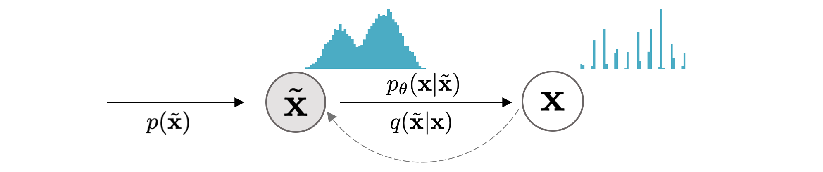
\includegraphics[width=\textwidth]{images/general.pdf}
    \caption[c]{Overview of the method \\ 
    ($\tilde{\bm{x}}$ --- the smoothed data, $q(\tilde{\bm{x}} \mid \bm{x})$ --- the smoothing distribution) \cite{orig}}
\end{figure}
\end{frame}

\section{Problems}
\begin{frame}
\frametitle{Problem 1: Manifold hypothesis}
Many real world data distributions (e.g.natural images) 
\newline
\textbf{may lie in the vicinity of a low-dimensional manifold} and can often \textbf{have complicated densities with sharp transitions} (i.e. high Lipschitz constants) that are difficult to model.
\begin{figure}[h]
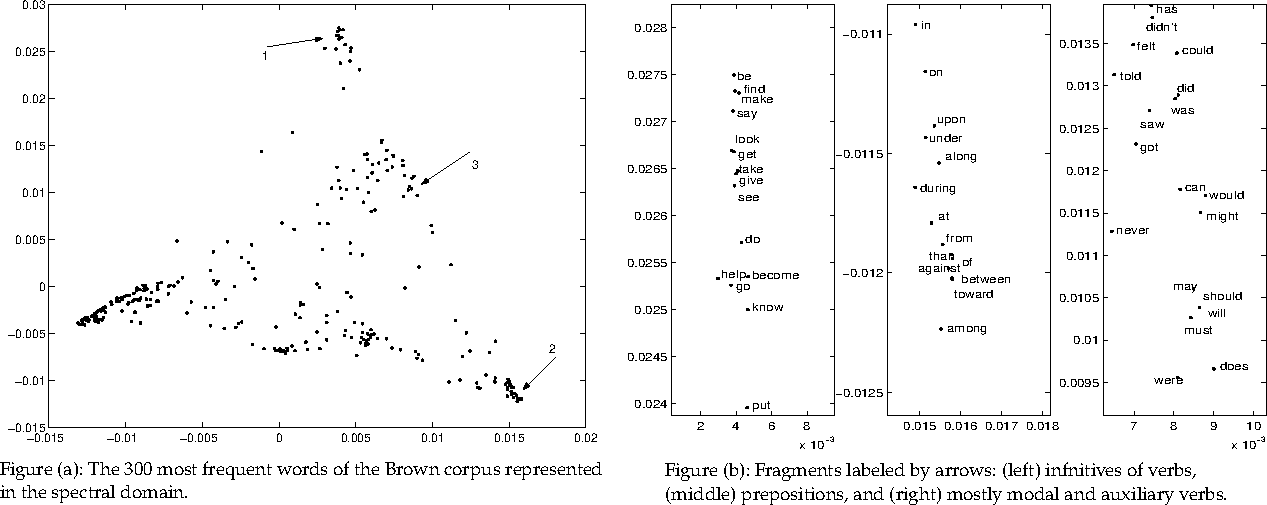
\includegraphics[width=\textwidth]{images/laplas.pdf}
\source{(Belkin M., Niyogi P., 2003) \cite{laplas}}
\end{figure}
\end{frame}

\begin{frame}[c]
\frametitle{Problem 1: Manifold hypothesis}
\begin{figure}[hp]

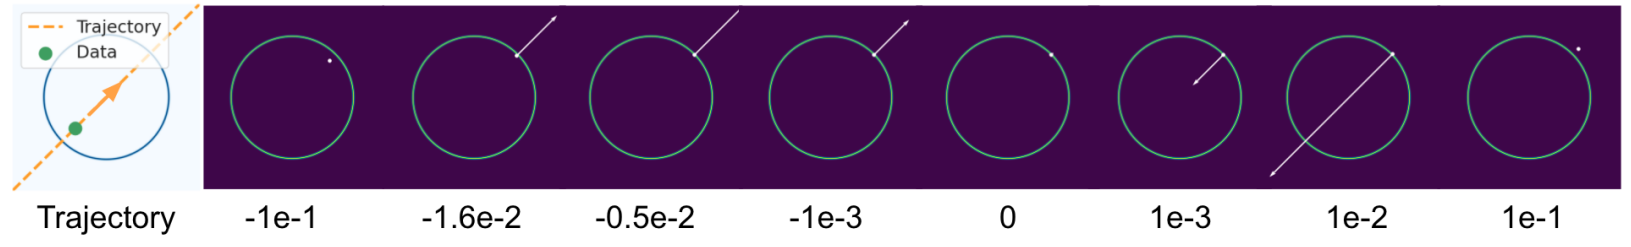
\includegraphics[width=\textwidth]{images/sharp.png}
\caption{ Ring distribution (almost a unit circle) formed by rotating the 1-d Gaussian distribution $\mathcal{N}\left(1,0.01^{2}\right)$ around the origin. The data location for each figure is $(\sqrt{0.5}+c, \sqrt{0.5}+c),$ where $c$ is the number below each figure and $(\sqrt{0.5}, \sqrt{0.5})$ is the upper right intersection of the trajectory with the unit circle. \cite{orig}
}
\end{figure}
\end{frame}

\begin{frame}[h]
\frametitle{Problem 2: Compounding errors}
$$
p(\bm{x})=\prod_{i=1}^{D} p\left(x_{i} \mid \bm{x}_{<i}\right)
$$
Compounding errors \textbf{comes from the inaccurate approximation of the conditional distributions.}  
\newline
\newline
The reasons for this may be:
\begin{itemize}
\item Curse of dimensionality + very limited amount of training data (in some cases)
\item The current state is based on the values of the previous states
\item Adversarial attacks
\end{itemize}
\end{frame}

\section{Theory \cite{orig}}
\begin{frame}[t]
\textbf{Theorem 1} Let: 
\begin{enumerate}
    \item $p(x)$ --- a continuous 1-d distribution that is supported on $\bm{R}$
    \item $q(\tilde{x} \mid x)$ --- 1-d distribution that is:
    \begin{itemize}
        \item symmetric (i.e. $q(\tilde{x} \mid x)=q(x \mid \tilde{x})$ )
        \item stationary (i.e. translation invariant)
        \item $\lim _{x \rightarrow \infty} p(x) q(x \mid \tilde{x})=0$ for any given $\tilde{x}$
    \end{itemize}
\end{enumerate}
\underline{Then}:
$\operatorname{Lip}(q(\tilde{x})) \leq \operatorname{Lip}\left(p_{\text {data }}(x)\right)$,

where $q(\tilde{x}) \triangleq \int q(\tilde{x} \mid x) p(x) d x$ and $\operatorname{Lip}(\cdot)$ denotes the Lipschitz constant of the given $1-d$ function.

\begin{figure}[h]

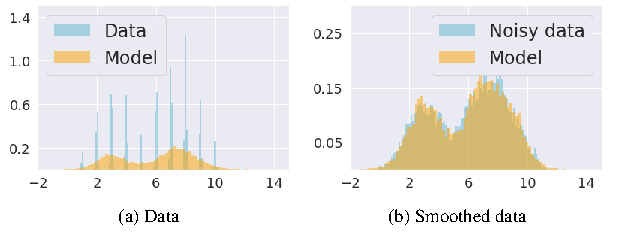
\includegraphics[scale=1]{images/ill_th1.pdf}
\caption{ Illustration of Theorem 1 \cite{orig}}
\end{figure}
\end{frame}

\begin{frame}
\textbf{Proposition 1} (Informal) Let: 
\begin{enumerate}
    \item $q(\tilde{\bm{x}} \mid \bm{x})$  is such that:
    \begin{itemize}
        \item symmetric
        \item stationary
        \item has small variance
        \item has negligible higher order moments (i.e. very small)
    \end{itemize}
\end{enumerate}
\underline{Then}:
$$
\bm{E}_{p_{\text {data }}(\bm{x})} \bm{E}_{q(\tilde{\bm{x}} \mid \bm{x})}\left[\log p_{\theta}(\tilde{\bm{x}})\right] \approx \bm{E}_{p_{\text {data }}(\bm{x})}\left[\log p_{\theta}(\bm{x})+\frac{\eta}{2} \sum_{i} \frac{\partial^{2} \log p_{\theta}}{\partial x_{i}^{2}}\right]
$$
for some constant $\eta .$ 
\newline
\newline
Since the samples from $p_{\text {data }}$ should be close to a local maximum of the model, this encourages the second order gradients computed at a data point $\bm{x}$ to become closer to zero (if it were positive then $\bm{x}$ will not be a local maximum), creating a smoothing effect.
\end{frame}

\begin{frame}[h]
\frametitle{Introducing $2^{nd}$ distribution: $p_{\theta}(\bm{x} \mid \tilde{\bm{x}})$}
\textcolor{blue}{Case 1} $q(\tilde{\bm{x}} \mid \bm{x})=\mathcal{N}\left(\tilde{\bm{x}} \mid \bm{x}, \sigma^{2} I\right)$ and $\sigma$ is small
\begin{block}{Single-step denoising \cite{single_step}}
\footnotesize
$
\overline{\bm{x}}=\tilde{\bm{x}}+\sigma^{2} \nabla_{\tilde{\bm{x}}} \log p_{\theta}(\tilde{\bm{x}})
$
\end{block}

\begin{figure}[ht]
        \begin{minipage}[b]{0.45\linewidth}
            \centering
            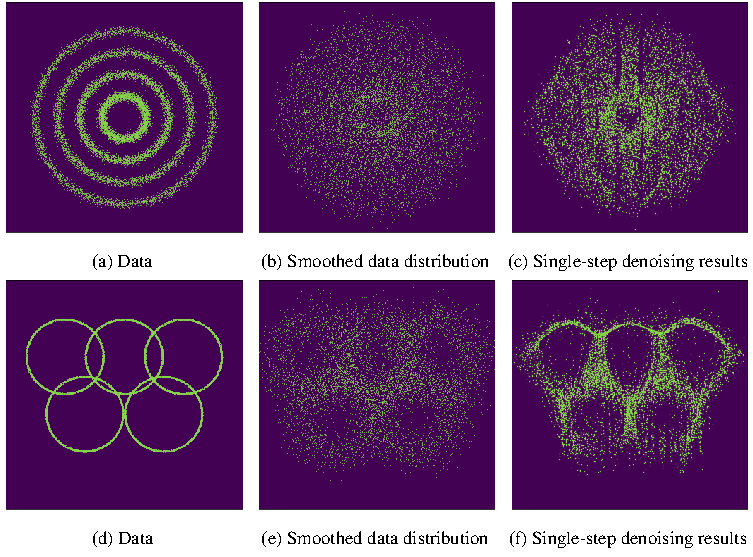
\includegraphics[width=\textwidth]{single_step.pdf}
            \caption{Example of "single-step denoising"}
        \end{minipage}
        \hspace{0.2cm}
        \begin{minipage}[b]{0.45\linewidth}
            \centering
            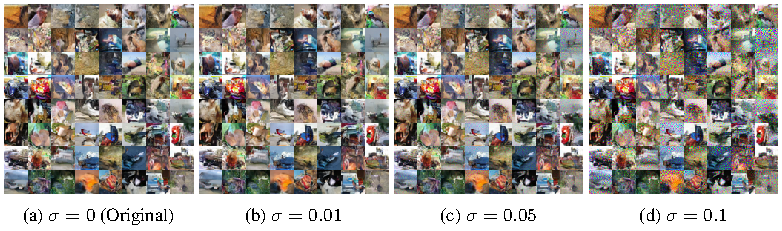
\includegraphics[width=\textwidth]{impl_single_step.pdf}
            \caption{"Single-step denoising" on PixelCNN++ trained on unsmoothed data}
        \end{minipage}
    \end{figure}

\end{frame}


\begin{frame}
\textcolor{blue}{Case 2} General case
\begin{block}{Maximizing an evidence lower bound (ELBO)\footnote{\href{https://lilianweng.github.io/lil-log/2018/08/12/from-autoencoder-to-beta-vae.html#autoencoder}{Formula derivation}}}
\footnotesize
$
\log p_{\theta}(\bm{x}) \geq \mathbb{E}_{p_{\text {data }}(\bm{x})}\left[\mathbb{E}_{q(\tilde{\bm{x}} \mid \bm{x})}\left[\log p_{\theta}(\tilde{\bm{x}})\right]-\mathbb{E}_{q(\tilde{\bm{x}} \mid \bm{x})}[\log q(\tilde{\bm{x}} \mid \bm{x})]+\mathbb{E}_{q(\tilde{\bm{x}} \mid \bm{x})}\left[\log p_{\theta}(\bm{x} \mid \tilde{\bm{x}})\right]\right]
$
\end{block}
\begin{figure}[h]
    \centering
    
    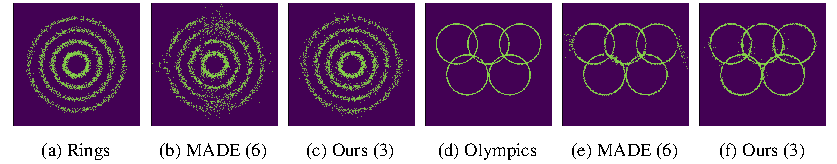
\includegraphics[width=\textwidth]{rings.pdf}
    \caption[c]{We use a MADE model with comparable number of parameters for both our method and the baseline}
\end{figure}
\begin{figure}[h]
    \centering
    
    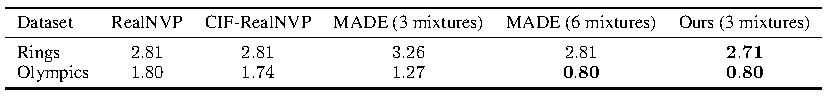
\includegraphics[width=\textwidth]{nll_rings.pdf}
    \caption[c]{Negative  log-likelihoods  on  2-d  synthetic  datasets  (lower  is  better)) }
\end{figure}
\end{frame}

\section{Experiments \cite{orig}}
\begin{frame}{Choosing  the smoothing distribution}
\begin{figure}[h]
    \centering
    
    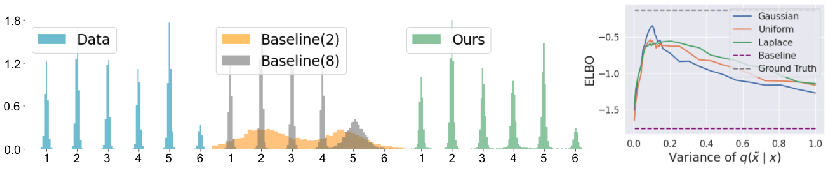
\includegraphics[width=\textwidth]{distrs.pdf}
    \caption[c]{Density estimation on 1-d synthetic dataset.  In the second figure, the digit in the paren-thesis denotes the number of mixture components used in the baseline mixture of logistics model.}
\end{figure}
For each type of distribution, we perform a grid search to find the optimal variance. Since our approach requires the modeling of both $p_{\theta}(\tilde{\bm{x}})$ and $p_{\theta}(\bm{x} \mid \tilde{\bm{x}}),$ we stack $\tilde{\bm{x}}$ and $\bm{x}$ together, and \newline
\emph{use a MADE model \cite{MADE} with a mixture of two logistic components} to parameterize $p_{\theta}(\tilde{\bm{x}})$ and $p_{\theta}(\bm{x} \mid \tilde{\bm{x}})$ at the same time. For the baseline model, we train a mixture of logistics model directly on $p_{\text {data }}(\bm{x})$.
\end{frame}

\begin{frame}
\begin{figure}[h]
    \centering
    
    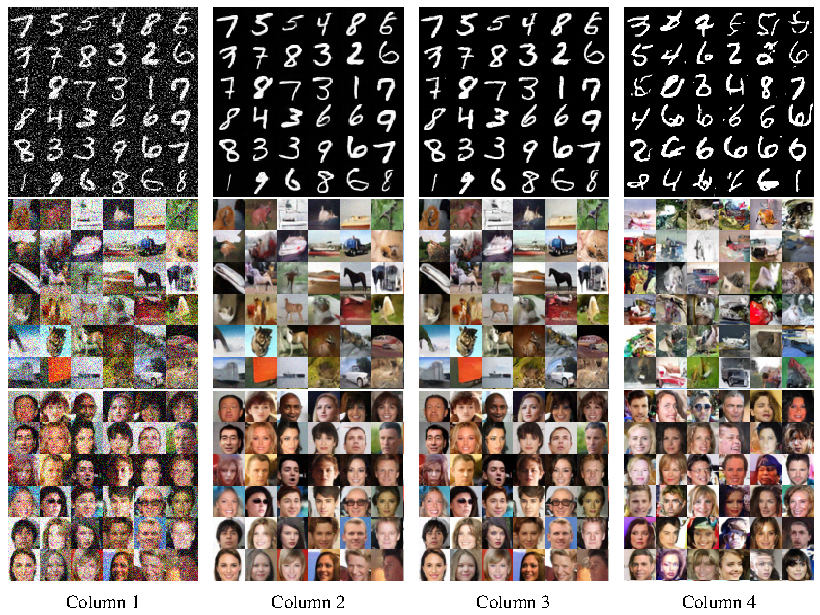
\includegraphics[scale=0.65]{columns.pdf}
    \caption[c]{From left to right: \textbf{Column 1}: samples from $p_{\theta}(\tilde{\bm{x}})$. \textbf{Column 2}: "single-step denoising" samples from $p_{\theta}(\tilde{\bm{x}}) .$ \textbf{Column 3} $\bm{3}:$ samples from $p_{\theta}(\bm{x} \mid \tilde{\bm{x}}) .$ \textbf{Column 4}: samples from the baseline PixelCNN++ model with parameters comparable to the sum of total parameters of $p_{\theta}(\tilde{\bm{x}})$ and $p_{\theta}(\bm{x} \mid \tilde{\bm{x}})$. }
\end{figure}
\end{frame}

\begin{frame}
\begin{figure}[h]
    \centering
    
    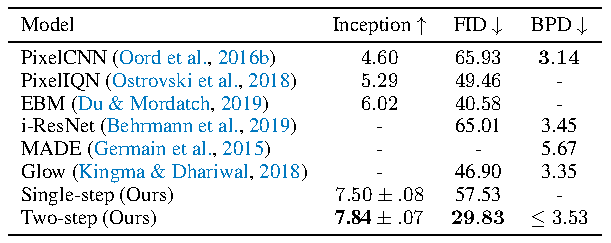
\includegraphics{scores.pdf}
    \caption[c]{Trained on unconditional CIFAR-10. Inception (higher is better) and FID scores (lower is better). "Single-step" samples are generated solely by $p_{\theta}(\tilde{\bm{x}})$. "Two-step" samples are generated by drawing samples from $p_{\theta}(\tilde{\bm{x}})$ and then "denoised" by $p_{\theta}(\bm{x} \mid \tilde{\bm{x}})$.}
\end{figure}
We use PixelCNN++ \href{https://arxiv.org/pdf/1701.05517.pdf}{\textcolor{blue}{(Salimans et al., 2017)}} as the model architecture for both $p_{\theta}(\tilde{\bm{x}})$ and $p_{\theta}(\bm{x} \mid \tilde{\bm{x}}).$
\end{frame}

\begin{frame}
\begin{figure}[h]
    \centering
    
    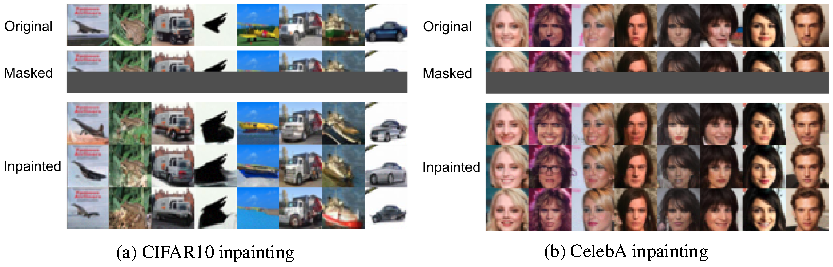
\includegraphics[width=\textwidth]{inpaintings.pdf}
    \caption[c]{Inpainting results from our two-step method}
\end{figure}
\footnotesize\begin{center}
\begin{figure}[h]
    \centering
    
    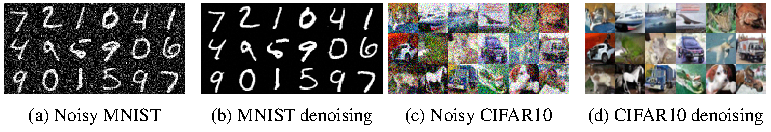
\includegraphics[width=\textwidth]{unnoise.pdf}
    \caption[c]{\text {Denoising with} p_{\theta}(\bm{x} \mid \tilde{\bm{x}})}
\end{figure}
\end{center}
\end{frame}

\begin{frame}{Normalizing flows \cite{nvp}}
\begin{figure}[h]
    \centering
    
    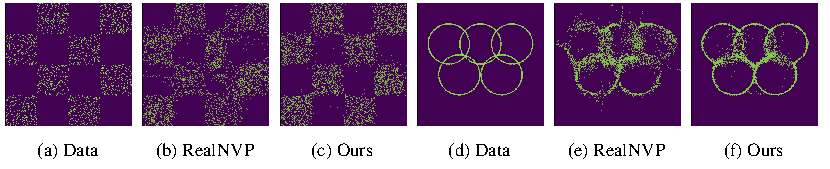
\includegraphics[width=\textwidth]{flows.pdf}
    \caption[c]{We compare the RealNVP model trained with randomize smoothing, where we use $p_{\theta}(\bm{x} \mid \tilde{\bm{x}})$ (also a RealNVP) to revert the smoothing process, with a RealNVP trained with the original method but with comparable number of parameters.}
\end{figure}
\footnotesize\begin{center}
\begin{tabular}{|c|c|c|c|}
\hline Model/Dataset & checkerboard & Olympics  \\
\hline Original & 3.72 & 1.80 \\
\hline Ours & \textbf{3.64} & \textbf{1.32} \\
\hline
\end{tabular}
\captionof{table}{NLL on the datasets. Distribution are modeled as RealNVP}
\end{center}
\end{frame}


\bibliographystyle{unsrt}
\bibliography{links}


\end{document}